\documentclass[14pt]{extbook}
\usepackage{multicol, enumerate, enumitem, hyperref, color, soul, setspace, parskip, fancyhdr} %General Packages
\usepackage{amssymb, amsthm, amsmath, bbm, latexsym, units, mathtools} %Math Packages
\everymath{\displaystyle} %All math in Display Style
% Packages with additional options
\usepackage[headsep=0.5cm,headheight=12pt, left=1 in,right= 1 in,top= 1 in,bottom= 1 in]{geometry}
\usepackage[usenames,dvipsnames]{xcolor}
\usepackage{dashrule}  % Package to use the command below to create lines between items
\newcommand{\litem}[1]{\item#1\hspace*{-1cm}\rule{\textwidth}{0.4pt}}
\pagestyle{fancy}
\lhead{Progress Quiz 5}
\chead{}
\rhead{Version C}
\lfoot{9912-2038}
\cfoot{}
\rfoot{Spring 2021}
\begin{document}

\begin{enumerate}
\litem{
What is the domain of the function below?\[ f(x) = \sqrt[8]{-4 x + 6} \]\begin{enumerate}[label=\Alph*.]
\item \( (-\infty, a], \text{where } a \in [0.28, 1.23] \)
\item \( [a, \infty), \text{where } a \in [0.35, 1.16] \)
\item \( (-\infty, \infty) \)
\item \( (-\infty, a], \text{ where } a \in [0.93, 1.55] \)
\item \( [a, \infty), \text{where } a \in [1.4, 1.66] \)

\end{enumerate} }
\litem{
Choose the graph of the equation below.\[ f(x) = - \sqrt{x - 14} - 7 \]\begin{enumerate}[label=\Alph*.]
\begin{multicols}{2}\item 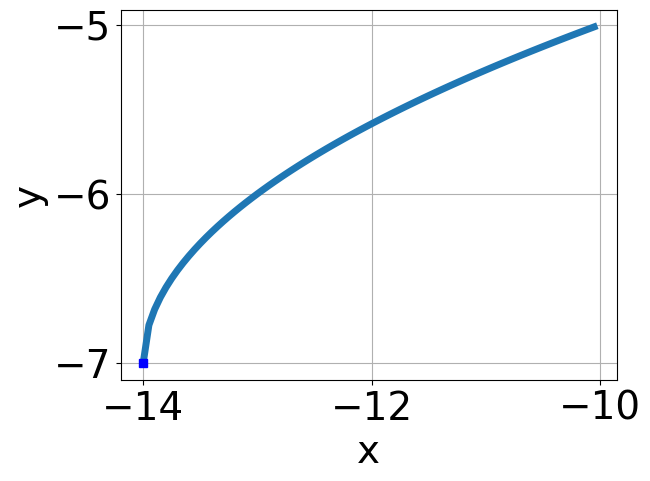
\includegraphics[width = 0.3\textwidth]{../Figures/radicalEquationToGraphAC.png}\item 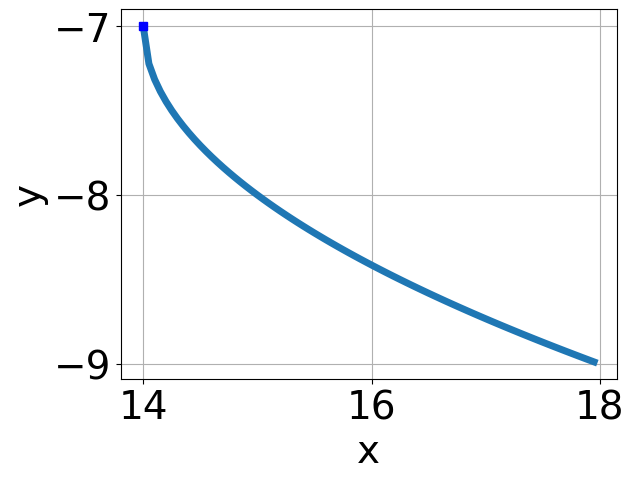
\includegraphics[width = 0.3\textwidth]{../Figures/radicalEquationToGraphBC.png}\item 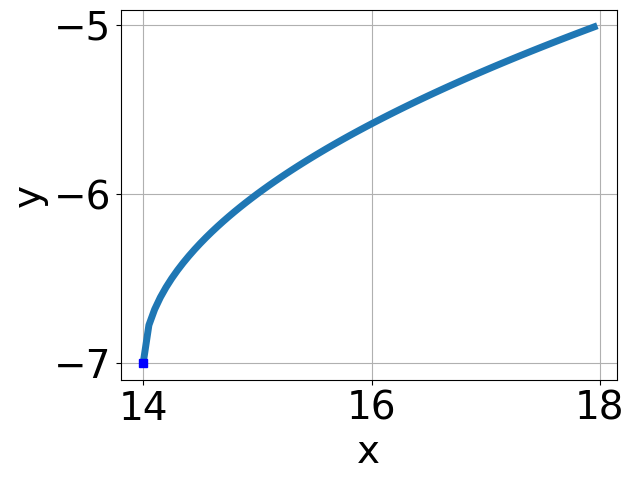
\includegraphics[width = 0.3\textwidth]{../Figures/radicalEquationToGraphCC.png}\item 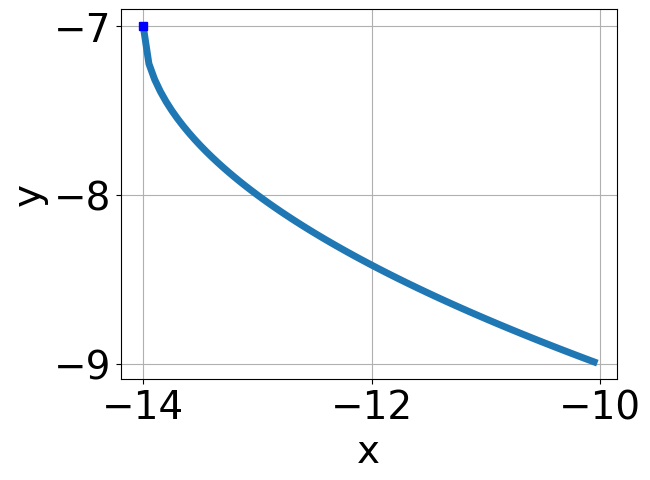
\includegraphics[width = 0.3\textwidth]{../Figures/radicalEquationToGraphDC.png}\end{multicols}\item None of the above.
\end{enumerate} }
\litem{
Solve the radical equation below. Then, choose the interval(s) that the solution(s) belongs to.\[ \sqrt{-9 x + 3} - \sqrt{-3 x + 6} = 0 \]\begin{enumerate}[label=\Alph*.]
\item \( x \in [-1.12,-0.34] \)
\item \( x \in [0.89,2.99] \)
\item \( x_1 \in [-0.42, 1.02] \text{ and } x_2 \in [1,6] \)
\item \( \text{All solutions lead to invalid or complex values in the equation.} \)
\item \( x_1 \in [-1.12, -0.34] \text{ and } x_2 \in [-0.67,1.33] \)

\end{enumerate} }
\litem{
Solve the radical equation below. Then, choose the interval(s) that the solution(s) belongs to.\[ \sqrt{-16 x^2 + 21} - \sqrt{-10 x} = 0 \]\begin{enumerate}[label=\Alph*.]
\item \( \text{All solutions lead to invalid or complex values in the equation.} \)
\item \( x_1 \in [-1.33, -0.03] \text{ and } x_2 \in [-1.5,2.5] \)
\item \( x \in [1.37,1.55] \)
\item \( x_1 \in [0.44, 0.95] \text{ and } x_2 \in [-1.5,2.5] \)
\item \( x \in [-1.33,-0.03] \)

\end{enumerate} }
\litem{
Solve the radical equation below. Then, choose the interval(s) that the solution(s) belongs to.\[ \sqrt{6 x - 2} - \sqrt{7 x + 7} = 0 \]\begin{enumerate}[label=\Alph*.]
\item \( x \in [-14,-5] \)
\item \( x \in [2,9] \)
\item \( x_1 \in [-1, 0] \text{ and } x_2 \in [0.33,3.33] \)
\item \( \text{All solutions lead to invalid or complex values in the equation.} \)
\item \( x_1 \in [-14, -5] \text{ and } x_2 \in [0.33,3.33] \)

\end{enumerate} }
\litem{
Choose the graph of the equation below.\[ f(x) = - \sqrt{x - 8} - 7 \]\begin{enumerate}[label=\Alph*.]
\begin{multicols}{2}\item 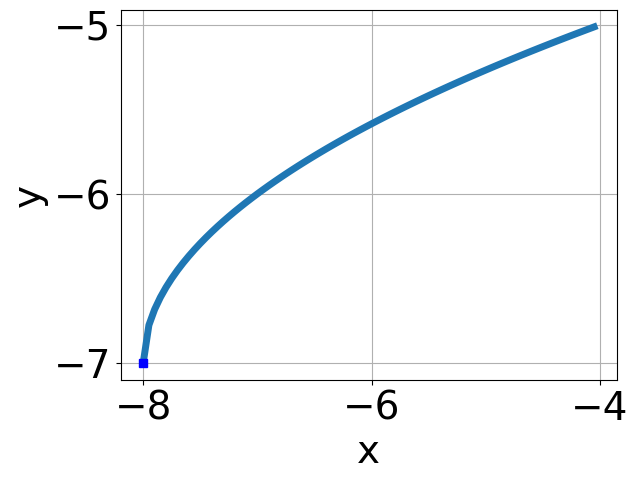
\includegraphics[width = 0.3\textwidth]{../Figures/radicalEquationToGraphCopyAC.png}\item 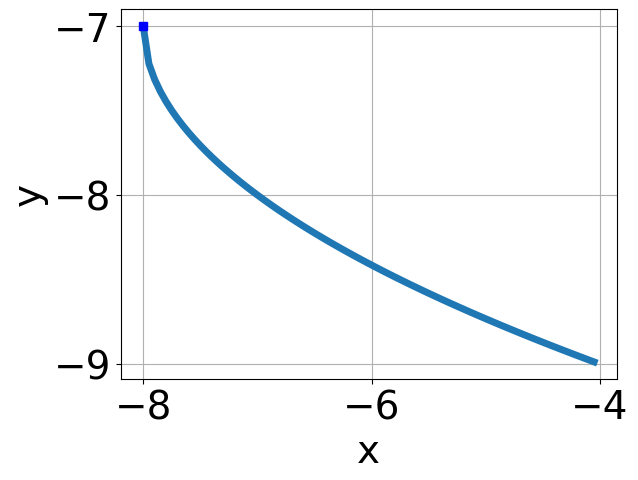
\includegraphics[width = 0.3\textwidth]{../Figures/radicalEquationToGraphCopyBC.png}\item 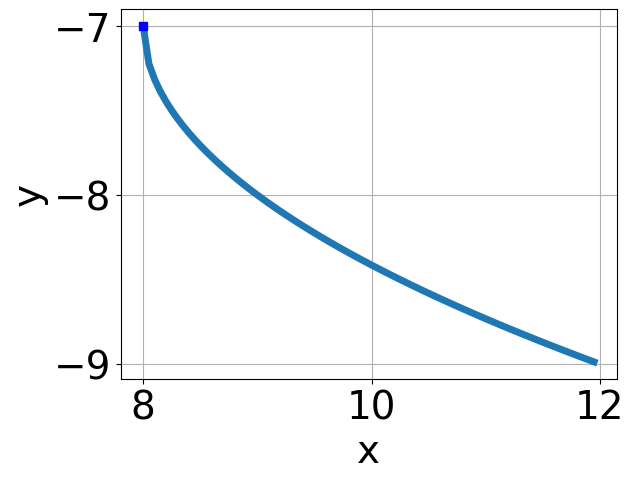
\includegraphics[width = 0.3\textwidth]{../Figures/radicalEquationToGraphCopyCC.png}\item 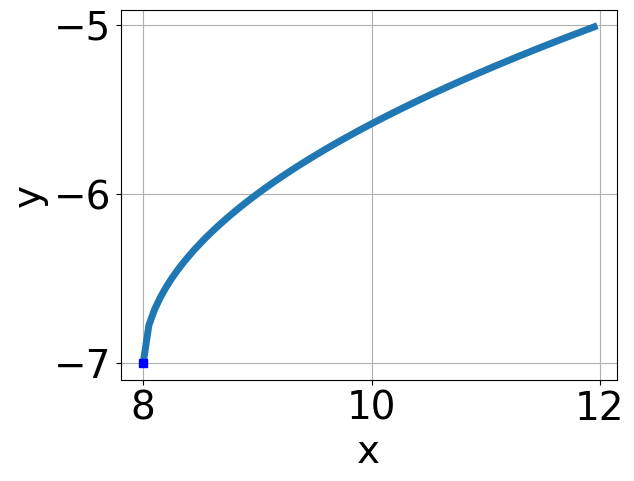
\includegraphics[width = 0.3\textwidth]{../Figures/radicalEquationToGraphCopyDC.png}\end{multicols}\item None of the above.
\end{enumerate} }
\litem{
Choose the equation of the function graphed below.
\begin{center}
    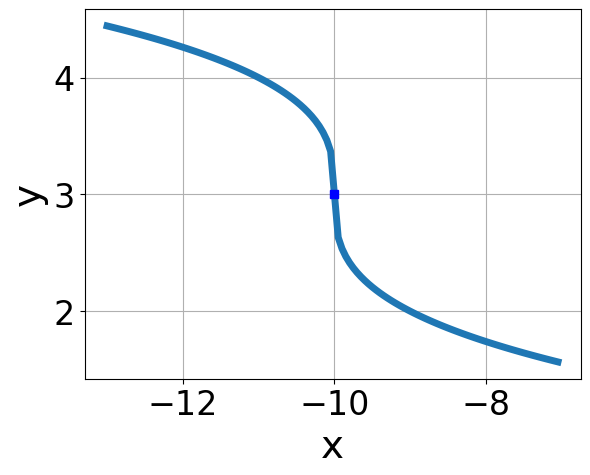
\includegraphics[width=0.5\textwidth]{../Figures/radicalGraphToEquationCopyC.png}
\end{center}
\begin{enumerate}[label=\Alph*.]
\item \( f(x) = \sqrt{x - 10} + 3 \)
\item \( f(x) = \sqrt{x + 10} + 3 \)
\item \( f(x) = - \sqrt{x - 10} + 3 \)
\item \( f(x) = - \sqrt{x + 10} + 3 \)
\item \( \text{None of the above} \)

\end{enumerate} }
\litem{
Solve the radical equation below. Then, choose the interval(s) that the solution(s) belongs to.\[ \sqrt{12 x^2 + 32} - \sqrt{-40 x} = 0 \]\begin{enumerate}[label=\Alph*.]
\item \( x_1 \in [0.69, 1.49] \text{ and } x_2 \in [-1,4] \)
\item \( \text{All solutions lead to invalid or complex values in the equation.} \)
\item \( x_1 \in [-2.98, -1.94] \text{ and } x_2 \in [-4.33,-0.33] \)
\item \( x \in [-1.34,-0.88] \)
\item \( x \in [-2.98,-1.94] \)

\end{enumerate} }
\litem{
What is the domain of the function below?\[ f(x) = \sqrt[8]{-4 x - 7} \]\begin{enumerate}[label=\Alph*.]
\item \( (-\infty, \infty) \)
\item \( (-\infty, a], \text{where } a \in [-0.7, 1.7] \)
\item \( [a, \infty), \text{where } a \in [-2.75, -0.75] \)
\item \( [a, \infty), \text{where } a \in [-1.57, 4.43] \)
\item \( (-\infty, a], \text{ where } a \in [-2.2, -1.1] \)

\end{enumerate} }
\litem{
Choose the equation of the function graphed below.
\begin{center}
    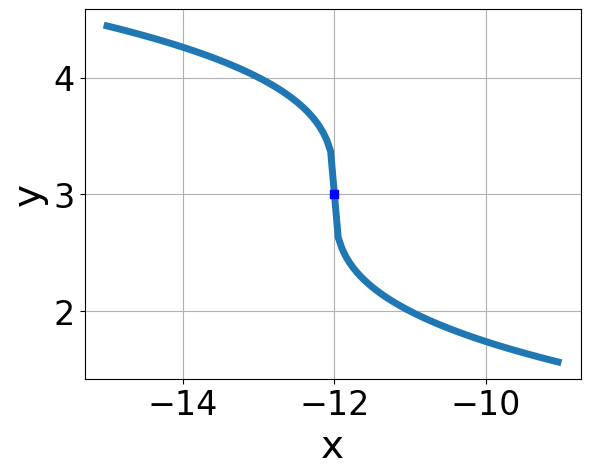
\includegraphics[width=0.5\textwidth]{../Figures/radicalGraphToEquationC.png}
\end{center}
\begin{enumerate}[label=\Alph*.]
\item \( f(x) = - \sqrt{x - 12} + 3 \)
\item \( f(x) = \sqrt{x - 12} + 3 \)
\item \( f(x) = - \sqrt{x + 12} + 3 \)
\item \( f(x) = \sqrt{x + 12} + 3 \)
\item \( \text{None of the above} \)

\end{enumerate} }
\end{enumerate}

\end{document}